\documentclass{beamer}
\usepackage[utf8]{inputenc}
\usepackage{verbatim}
\usepackage{fancyvrb}
\usepackage{color}
\usepackage{tikz}

\makeatletter
\def\PY@reset{\let\PY@it=\relax \let\PY@bf=\relax%
    \let\PY@ul=\relax \let\PY@tc=\relax%
    \let\PY@bc=\relax \let\PY@ff=\relax}
\def\PY@tok#1{\csname PY@tok@#1\endcsname}
\def\PY@toks#1+{\ifx\relax#1\empty\else%
    \PY@tok{#1}\expandafter\PY@toks\fi}
\def\PY@do#1{\PY@bc{\PY@tc{\PY@ul{%
    \PY@it{\PY@bf{\PY@ff{#1}}}}}}}
\def\PY#1#2{\PY@reset\PY@toks#1+\relax+\PY@do{#2}}

\expandafter\def\csname PY@tok@gd\endcsname{\def\PY@tc##1{\textcolor[rgb]{0.63,0.00,0.00}{##1}}}
\expandafter\def\csname PY@tok@gu\endcsname{\let\PY@bf=\textbf\def\PY@tc##1{\textcolor[rgb]{0.50,0.00,0.50}{##1}}}
\expandafter\def\csname PY@tok@gt\endcsname{\def\PY@tc##1{\textcolor[rgb]{0.00,0.25,0.82}{##1}}}
\expandafter\def\csname PY@tok@gs\endcsname{\let\PY@bf=\textbf}
\expandafter\def\csname PY@tok@gr\endcsname{\def\PY@tc##1{\textcolor[rgb]{1.00,0.00,0.00}{##1}}}
\expandafter\def\csname PY@tok@cm\endcsname{\let\PY@it=\textit\def\PY@tc##1{\textcolor[rgb]{0.25,0.50,0.50}{##1}}}
\expandafter\def\csname PY@tok@vg\endcsname{\def\PY@tc##1{\textcolor[rgb]{0.10,0.09,0.49}{##1}}}
\expandafter\def\csname PY@tok@m\endcsname{\def\PY@tc##1{\textcolor[rgb]{0.40,0.40,0.40}{##1}}}
\expandafter\def\csname PY@tok@mh\endcsname{\def\PY@tc##1{\textcolor[rgb]{0.40,0.40,0.40}{##1}}}
\expandafter\def\csname PY@tok@go\endcsname{\def\PY@tc##1{\textcolor[rgb]{0.50,0.50,0.50}{##1}}}
\expandafter\def\csname PY@tok@ge\endcsname{\let\PY@it=\textit}
\expandafter\def\csname PY@tok@vc\endcsname{\def\PY@tc##1{\textcolor[rgb]{0.10,0.09,0.49}{##1}}}
\expandafter\def\csname PY@tok@il\endcsname{\def\PY@tc##1{\textcolor[rgb]{0.40,0.40,0.40}{##1}}}
\expandafter\def\csname PY@tok@cs\endcsname{\let\PY@it=\textit\def\PY@tc##1{\textcolor[rgb]{0.25,0.50,0.50}{##1}}}
\expandafter\def\csname PY@tok@cp\endcsname{\def\PY@tc##1{\textcolor[rgb]{0.74,0.48,0.00}{##1}}}
\expandafter\def\csname PY@tok@gi\endcsname{\def\PY@tc##1{\textcolor[rgb]{0.00,0.63,0.00}{##1}}}
\expandafter\def\csname PY@tok@gh\endcsname{\let\PY@bf=\textbf\def\PY@tc##1{\textcolor[rgb]{0.00,0.00,0.50}{##1}}}
\expandafter\def\csname PY@tok@ni\endcsname{\let\PY@bf=\textbf\def\PY@tc##1{\textcolor[rgb]{0.60,0.60,0.60}{##1}}}
\expandafter\def\csname PY@tok@nl\endcsname{\def\PY@tc##1{\textcolor[rgb]{0.63,0.63,0.00}{##1}}}
\expandafter\def\csname PY@tok@nn\endcsname{\let\PY@bf=\textbf\def\PY@tc##1{\textcolor[rgb]{0.00,0.00,1.00}{##1}}}
\expandafter\def\csname PY@tok@no\endcsname{\def\PY@tc##1{\textcolor[rgb]{0.53,0.00,0.00}{##1}}}
\expandafter\def\csname PY@tok@na\endcsname{\def\PY@tc##1{\textcolor[rgb]{0.49,0.56,0.16}{##1}}}
\expandafter\def\csname PY@tok@nb\endcsname{\def\PY@tc##1{\textcolor[rgb]{0.00,0.50,0.00}{##1}}}
\expandafter\def\csname PY@tok@nc\endcsname{\let\PY@bf=\textbf\def\PY@tc##1{\textcolor[rgb]{0.00,0.00,1.00}{##1}}}
\expandafter\def\csname PY@tok@nd\endcsname{\def\PY@tc##1{\textcolor[rgb]{0.67,0.13,1.00}{##1}}}
\expandafter\def\csname PY@tok@ne\endcsname{\let\PY@bf=\textbf\def\PY@tc##1{\textcolor[rgb]{0.82,0.25,0.23}{##1}}}
\expandafter\def\csname PY@tok@nf\endcsname{\def\PY@tc##1{\textcolor[rgb]{0.00,0.00,1.00}{##1}}}
\expandafter\def\csname PY@tok@si\endcsname{\let\PY@bf=\textbf\def\PY@tc##1{\textcolor[rgb]{0.73,0.40,0.53}{##1}}}
\expandafter\def\csname PY@tok@s2\endcsname{\def\PY@tc##1{\textcolor[rgb]{0.73,0.13,0.13}{##1}}}
\expandafter\def\csname PY@tok@vi\endcsname{\def\PY@tc##1{\textcolor[rgb]{0.10,0.09,0.49}{##1}}}
\expandafter\def\csname PY@tok@nt\endcsname{\let\PY@bf=\textbf\def\PY@tc##1{\textcolor[rgb]{0.00,0.50,0.00}{##1}}}
\expandafter\def\csname PY@tok@nv\endcsname{\def\PY@tc##1{\textcolor[rgb]{0.10,0.09,0.49}{##1}}}
\expandafter\def\csname PY@tok@s1\endcsname{\def\PY@tc##1{\textcolor[rgb]{0.73,0.13,0.13}{##1}}}
\expandafter\def\csname PY@tok@sh\endcsname{\def\PY@tc##1{\textcolor[rgb]{0.73,0.13,0.13}{##1}}}
\expandafter\def\csname PY@tok@sc\endcsname{\def\PY@tc##1{\textcolor[rgb]{0.73,0.13,0.13}{##1}}}
\expandafter\def\csname PY@tok@sx\endcsname{\def\PY@tc##1{\textcolor[rgb]{0.00,0.50,0.00}{##1}}}
\expandafter\def\csname PY@tok@bp\endcsname{\def\PY@tc##1{\textcolor[rgb]{0.00,0.50,0.00}{##1}}}
\expandafter\def\csname PY@tok@c1\endcsname{\let\PY@it=\textit\def\PY@tc##1{\textcolor[rgb]{0.25,0.50,0.50}{##1}}}
\expandafter\def\csname PY@tok@kc\endcsname{\let\PY@bf=\textbf\def\PY@tc##1{\textcolor[rgb]{0.00,0.50,0.00}{##1}}}
\expandafter\def\csname PY@tok@c\endcsname{\let\PY@it=\textit\def\PY@tc##1{\textcolor[rgb]{0.25,0.50,0.50}{##1}}}
\expandafter\def\csname PY@tok@mf\endcsname{\def\PY@tc##1{\textcolor[rgb]{0.40,0.40,0.40}{##1}}}
\expandafter\def\csname PY@tok@err\endcsname{\def\PY@bc##1{\setlength{\fboxsep}{0pt}\fcolorbox[rgb]{1.00,0.00,0.00}{1,1,1}{\strut ##1}}}
\expandafter\def\csname PY@tok@kd\endcsname{\let\PY@bf=\textbf\def\PY@tc##1{\textcolor[rgb]{0.00,0.50,0.00}{##1}}}
\expandafter\def\csname PY@tok@ss\endcsname{\def\PY@tc##1{\textcolor[rgb]{0.10,0.09,0.49}{##1}}}
\expandafter\def\csname PY@tok@sr\endcsname{\def\PY@tc##1{\textcolor[rgb]{0.73,0.40,0.53}{##1}}}
\expandafter\def\csname PY@tok@mo\endcsname{\def\PY@tc##1{\textcolor[rgb]{0.40,0.40,0.40}{##1}}}
\expandafter\def\csname PY@tok@kn\endcsname{\let\PY@bf=\textbf\def\PY@tc##1{\textcolor[rgb]{0.00,0.50,0.00}{##1}}}
\expandafter\def\csname PY@tok@mi\endcsname{\def\PY@tc##1{\textcolor[rgb]{0.40,0.40,0.40}{##1}}}
\expandafter\def\csname PY@tok@gp\endcsname{\let\PY@bf=\textbf\def\PY@tc##1{\textcolor[rgb]{0.00,0.00,0.50}{##1}}}
\expandafter\def\csname PY@tok@o\endcsname{\def\PY@tc##1{\textcolor[rgb]{0.40,0.40,0.40}{##1}}}
\expandafter\def\csname PY@tok@kr\endcsname{\let\PY@bf=\textbf\def\PY@tc##1{\textcolor[rgb]{0.00,0.50,0.00}{##1}}}
\expandafter\def\csname PY@tok@s\endcsname{\def\PY@tc##1{\textcolor[rgb]{0.73,0.13,0.13}{##1}}}
\expandafter\def\csname PY@tok@kp\endcsname{\def\PY@tc##1{\textcolor[rgb]{0.00,0.50,0.00}{##1}}}
\expandafter\def\csname PY@tok@w\endcsname{\def\PY@tc##1{\textcolor[rgb]{0.73,0.73,0.73}{##1}}}
\expandafter\def\csname PY@tok@kt\endcsname{\def\PY@tc##1{\textcolor[rgb]{0.69,0.00,0.25}{##1}}}
\expandafter\def\csname PY@tok@ow\endcsname{\let\PY@bf=\textbf\def\PY@tc##1{\textcolor[rgb]{0.67,0.13,1.00}{##1}}}
\expandafter\def\csname PY@tok@sb\endcsname{\def\PY@tc##1{\textcolor[rgb]{0.73,0.13,0.13}{##1}}}
\expandafter\def\csname PY@tok@k\endcsname{\let\PY@bf=\textbf\def\PY@tc##1{\textcolor[rgb]{0.00,0.50,0.00}{##1}}}
\expandafter\def\csname PY@tok@se\endcsname{\let\PY@bf=\textbf\def\PY@tc##1{\textcolor[rgb]{0.73,0.40,0.13}{##1}}}
\expandafter\def\csname PY@tok@sd\endcsname{\let\PY@it=\textit\def\PY@tc##1{\textcolor[rgb]{0.73,0.13,0.13}{##1}}}

\def\PYZbs{\char`\\}
\def\PYZus{\char`\_}
\def\PYZob{\char`\{}
\def\PYZcb{\char`\}}
\def\PYZca{\char`\^}
\def\PYZam{\char`\&}
\def\PYZlt{\char`\<}
\def\PYZgt{\char`\>}
\def\PYZsh{\char`\#}
\def\PYZpc{\char`\%}
\def\PYZdl{\char`\$}
\def\PYZti{\char`\~}
% for compatibility with earlier versions
\def\PYZat{@}
\def\PYZlb{[}
\def\PYZrb{]}
\makeatother

%\usetheme{default}
\begin{document}
\title{Workshop django}

\maketitle{}

\begin{frame}{Requirements}
\begin{itemize}
    \item savoir coder
    \item connaitre la programmation orienté objet
    \item python (la base)
    \item sql (pas forcement poussée)
    \item html (la base)
    \item regexp (la base)
    \item savoir utiliser un shell (la base)
\end{itemize}
\end{frame}

\begin{frame}{Introduction}
    C'est quoi django ?
    \begin{itemize}
        \item framework web en python\pause
        \item full stacked (vs microframework comme flask, bottle et les 15 milles autres)\pause
        \item vous "impose" un orm et un système de templates (changeable tous les 2 mais pas pensé pour)\pause
        \item mais en échange vous avez les django app\pause
        \item facile à utiliser (quasi tout), gros gain de productivité mais beaucoup à apprendre, vous allez souvent utiliser la documentation
    \end{itemize}
\end{frame}

\begin{frame}{Plan}
    \begin{itemize}
        \item Installation
        \item Hello world
        \item MTV basique
        \item Avancé ?
        \item Jquery ?
    \end{itemize}
\end{frame}

\begin{frame}{Installation}
2 façons de faire
\begin{itemize}
    \item la classique avec le pkg manager de la distribution (eg: sudo apt-get install django)
    \item en utilisant pypi via pip (on va utiliser celle là) dans un virtualenv
\end{itemize}
\end{frame}

\begin{frame}{Installation}
    Faire:
    \begin{itemize}
        \item Installation de pip (sudo apt-get install python-pip)\pause
        \item sudo pip install virtualenv (ou alors avec le package python-virtualenv)\pause
        \item aller dans un nouveau répertoire (mkdir blog \&\& cd blog)\pause
        \item virtualenv --no-site-packages --distribute ve\pause
        \item source ve/bin/activate \# pour rentrer dans le venv\pause
        \item pip install django\pause
        \item rehash \# pour zsh
    \end{itemize}
    \vspace{3mm}
    \pause
    Si vous voulez sortir du venv:
    \begin{itemize}
        \item deactivate
    \end{itemize}
\end{frame}

\begin{frame}[fragile]{Mon premier projet django}
    Faire dans le virtualenv:
            \begin{verbatim}
    django-admin.py startproject <nom du projet>
            \end{verbatim}
    \pause
    Lancer le serveur de développement:
    \begin{verbatim}
    cd <nom du projet> && python manage.py runserver
    \end{verbatim}
    Puis aller sur http://0.0.0.0:8000
\end{frame}

\begin{frame}[fragile]{Django 1.4}
    Vous allez obtenir une hiérarchie du style:

\begin{verbatim}
    project/urls.py
    project/settings.py
    project/__init__.py
    project/wsgi.py
    manage.py
\end{verbatim}

\end{frame}

\begin{frame}[fragile]{Django <= 1.3}
    Remarque: vous allez aussi rencontrer des projets ayant la forme suivante (django <= 1.3)
    \begin{verbatim}
    urls.py
    settings.py
    manage.py
    __init__.py
    \end{verbatim}
\end{frame}

\begin{frame}[fragile]{urls.py}
\begin{footnotesize}
\begin{Verbatim}[commandchars=\\\{\}]
\PY{k+kn}{from} \PY{n+nn}{django.conf.urls} \PY{k+kn}{import} \PY{n}{patterns}\PY{p}{,} \PY{n}{include}\PY{p}{,} \PY{n}{url}

\PY{c}{\PYZsh{} Uncomment the next two lines to enable the admin:}
\PY{c}{\PYZsh{} from django.contrib import admin}
\PY{c}{\PYZsh{} admin.autodiscover()}

\PY{n}{urlpatterns} \PY{o}{=} \PY{n}{patterns}\PY{p}{(}\PY{l+s}{'}\PY{l+s}{'}\PY{p}{,}
    \PY{c}{\PYZsh{} Examples:}
    \PY{c}{\PYZsh{} url(r'\PYZca{}\PYZdl{}', 'project.views.home', name='home'),}
    \PY{c}{\PYZsh{} url(r'\PYZca{}project/', include('project.foo.urls')),}

    \PY{c}{\PYZsh{} Uncomment the admin/doc line below to enable admin documentation:}
    \PY{c}{\PYZsh{} url(r'\PYZca{}admin/doc/', include('django.contrib.admindocs.urls')),}

    \PY{c}{\PYZsh{} Uncomment the next line to enable the admin:}
    \PY{c}{\PYZsh{} url(r'\PYZca{}admin/', include(admin.site.urls)),}
\PY{p}{)}
\end{Verbatim}
\end{footnotesize}
\end{frame}

\begin{frame}[fragile]{Hello World}
\begin{footnotesize}
\begin{Verbatim}[commandchars=\\\{\}]
\PY{k+kn}{from} \PY{n+nn}{django.conf.urls} \PY{k+kn}{import} \PY{n}{patterns}\PY{p}{,} \PY{n}{include}\PY{p}{,} \PY{n}{url}
\PY{k+kn}{from} \PY{n+nn}{django.http} \PY{k+kn}{import} \PY{n}{HttpResponse}

\PY{k}{def} \PY{n+nf}{hello}\PY{p}{(}\PY{n}{request}\PY{p}{)}\PY{p}{:}
    \PY{k}{return} \PY{n}{HttpResponse}\PY{p}{(}\PY{l+s}{"}\PY{l+s}{Hello World!}\PY{l+s}{"}\PY{p}{)}

\PY{n}{urlpatterns} \PY{o}{=} \PY{n}{patterns}\PY{p}{(}\PY{l+s}{'}\PY{l+s}{'}\PY{p}{,}
    \PY{n}{url}\PY{p}{(}\PY{l+s}{r'}\PY{l+s}{\PYZca{}\PYZdl{}}\PY{l+s}{'}\PY{p}{,} \PY{n}{hello}\PY{p}{)}\PY{p}{,}
\PY{p}{)}
\end{Verbatim}
\end{footnotesize}

Remarque: traditionnelement ces fonctions sont dans un fichier $views.py$

\end{frame}

\begin{frame}[fragile]{La vie d'une requète}

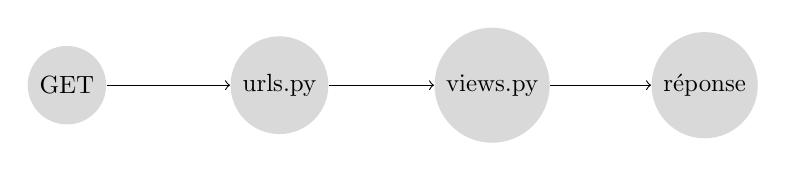
\begin{tikzpicture}[scale=.9, transform shape]
\tikzstyle{every node} = [circle, fill=gray!30]
\node (a) at (0, 0) {GET};
\node (b) at (3, 0) {urls.py};
\node (c) at (6, 0) {views.py};
\node (d) at (9, 0) {réponse};
\foreach \from/\to in {a/b, b/c, c/d}
\draw [->] (\from) -- (\to);
\end{tikzpicture}

\end{frame}

\begin{frame}[fragile]{MTV}

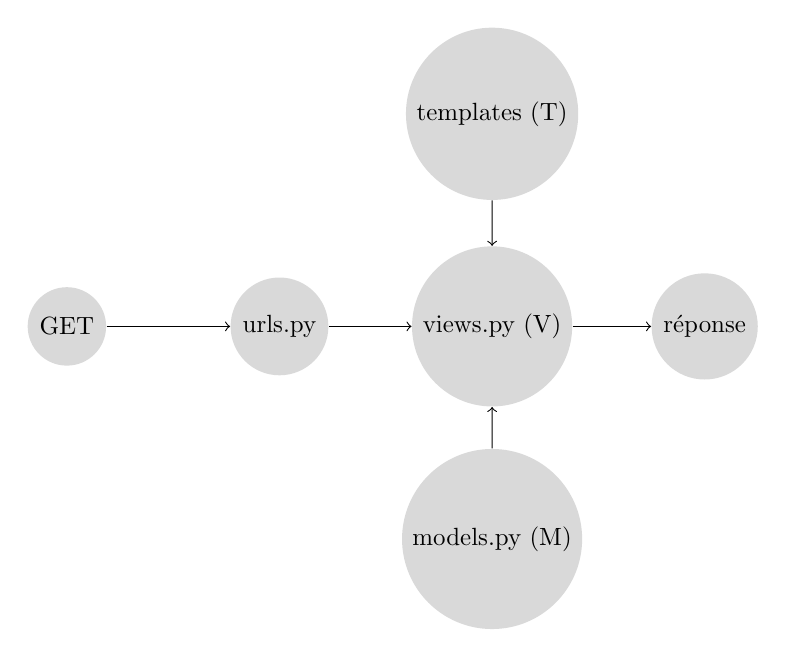
\begin{tikzpicture}[scale=.9, transform shape]
\tikzstyle{every node} = [circle, fill=gray!30]
\node (a) at (0, 0) {GET};
\node (b) at (3, 0) {urls.py};
\node (c) at (6, 0) {views.py (V)};
\node (e) at (6, 3) {templates (T)};
\node (f) at (6, -3) {models.py (M)};
\node (d) at (9, 0) {réponse};
\foreach \from/\to in {a/b, b/c, c/d, e/c, f/c}
\draw [->] (\from) -- (\to);
\end{tikzpicture}

\end{frame}

\begin{frame}[fragile]{Plan pour la partie mtv}
    \begin{itemize}
        \item urls.py
        \item templates
        \item models
        \item interface admin
    \end{itemize}
\end{frame}

\begin{frame}[fragile]{urls.py}
    Comment choper un argument:

\begin{footnotesize}
\begin{Verbatim}[commandchars=\\\{\}]
\PY{k+kn}{from} \PY{n+nn}{django.conf.urls} \PY{k+kn}{import} \PY{n}{patterns}\PY{p}{,} \PY{n}{include}\PY{p}{,} \PY{n}{url}
\PY{k+kn}{from} \PY{n+nn}{django.http} \PY{k+kn}{import} \PY{n}{HttpResponse}

\PY{o}{.}\PY{o}{.}\PY{o}{.}

\PY{k}{def} \PY{n+nf}{with\PYZus{}arg}\PY{p}{(}\PY{n}{request}\PY{p}{,} \PY{n}{argument}\PY{p}{)}\PY{p}{:}
    \PY{k}{return} \PY{n}{HttpResponse}\PY{p}{(}\PY{l+s}{"}\PY{l+s}{Hello }\PY{l+s+si}{\PYZpc{}s}\PY{l+s}{"} \PY{o}{\PYZpc{}} \PY{n}{argument}\PY{p}{)}

\PY{n}{urlpatterns} \PY{o}{=} \PY{n}{patterns}\PY{p}{(}\PY{l+s}{'}\PY{l+s}{'}\PY{p}{,}
    \PY{o}{.}\PY{o}{.}\PY{o}{.}
    \PY{n}{url}\PY{p}{(}\PY{l+s}{r'}\PY{l+s}{\PYZca{}(.*)/\PYZdl{}}\PY{l+s}{'}\PY{p}{,} \PY{n}{with\PYZus{}arg}\PY{p}{)}\PY{p}{,}
\PY{p}{)}
\end{Verbatim}
\end{footnotesize}

Pour tester aller sur $http://0.0.0.0:8000/world/$

\end{frame}

\begin{frame}[fragile]{Templates}
    Dans le répertoire de votre projet, au niveau où il y a le $manage.py$ faire:
    \begin{verbatim}
    mkdir templates
    \end{verbatim}
    Puis créer un fichier $templates/hello.html$ contenant:
    \begin{verbatim}
    <p>Hello {{ name }}</p>
    \end{verbatim}
\end{frame}

\begin{frame}[fragile]{Utiliser un template}
    Utiliser un template version moyen âge:

\begin{footnotesize}
\begin{Verbatim}[commandchars=\\\{\}]
\PY{k+kn}{from} \PY{n+nn}{django.template} \PY{k+kn}{import} \PY{n}{Context}\PY{p}{,} \PY{n}{loader}

\PY{k}{def} \PY{n+nf}{with\PYZus{}arg}\PY{p}{(}\PY{n}{request}\PY{p}{,} \PY{n}{argument}\PY{p}{)}\PY{p}{:}
    \PY{n}{t} \PY{o}{=} \PY{n}{loader}\PY{o}{.}\PY{n}{get\PYZus{}template}\PY{p}{(}\PY{l+s}{'}\PY{l+s}{hello.html}\PY{l+s}{'}\PY{p}{)}
    \PY{n}{c} \PY{o}{=} \PY{n}{Context}\PY{p}{(}\PY{p}{\PYZob{}}
        \PY{l+s}{'}\PY{l+s}{name}\PY{l+s}{'}\PY{p}{:} \PY{n}{argument}\PY{p}{,}
    \PY{p}{\PYZcb{}}\PY{p}{)}
    \PY{k}{return} \PY{n}{HttpResponse}\PY{p}{(}\PY{n}{t}\PY{o}{.}\PY{n}{render}\PY{p}{(}\PY{n}{c}\PY{p}{)}\PY{p}{)}
\end{Verbatim}
\end{footnotesize}

On utilisera \bf{jamais}  ça.
\end{frame}

\begin{frame}[fragile]{Utiliser un template}
    Ce que tout le monde utilise:

\begin{footnotesize}
\begin{Verbatim}[commandchars=\\\{\}]
\PY{k+kn}{from} \PY{n+nn}{django.shortcuts} \PY{k+kn}{import} \PY{n}{render}

\PY{k}{def} \PY{n+nf}{with\PYZus{}arg}\PY{p}{(}\PY{n}{request}\PY{p}{,} \PY{n}{argument}\PY{p}{)}\PY{p}{:}
    \PY{k}{return} \PY{n}{render}\PY{p}{(}\PY{n}{request}\PY{p}{,} \PY{l+s}{"}\PY{l+s}{hello.html}\PY{l+s}{"}\PY{p}{,} \PY{p}{\PYZob{}}\PY{l+s}{"}\PY{l+s}{name}\PY{l+s}{"}\PY{p}{:} \PY{n}{argument}\PY{p}{\PYZcb{}}\PY{p}{)}
\end{Verbatim}
\end{footnotesize}

\end{frame}

\begin{frame}[fragile]{Utiliser un template}
    Si vous essayez d'aller sur $http://0.0.0.0:8000/world/$ vous allez avoir une erreur $TemplateDoesNotExist at /world/$.

    \vspace{3mm}

    C'est parce que django demande qu'on lui dise où sont les templates (sauf pour les apps, cf plus tard).

    \vspace{3mm}

    Cela se fait dans le fichier $settings.py$.
\end{frame}

\begin{frame}[fragile]{Utiliser un template}
    Dans $settings.py$ chercher un truc qui ressemble à ça:

\begin{footnotesize}
    \begin{verbatim}
TEMPLATE_DIRS = (
    # Put strings here, like "/home/html/django_templates" or "C:/www/django/templates".
    # Always use forward slashes, even on Windows.
    # Don't forget to use absolute paths, not relative paths.
)
    \end{verbatim}
\end{footnotesize}\pause

Et mettre quelque chose du style:

\begin{footnotesize}
\begin{verbatim}
TEMPLATE_DIRS = (
    '/home/urlab/code/slides/workshop-django/1.4/project/templates',
)
\end{verbatim}
\end{footnotesize}\pause

Remarque: ce n'est pas portable, en vrai on utilise des paths relatifs, ici par simplicité je ne l'ai pas montré.\pause

\vspace{3mm}
\bf La virgule à la fin du string est OBLIGATOIRE sinon python ne considère pas que c'est un tuple.

\end{frame}

\begin{frame}[fragile]{Utiliser un template}
    Retourner sur $http://0.0.0.0:8000/world$, cela devrait fonctionner désormait.

    Remarque: vérifier que le serveur de dev se lance bien et qu'il ne montre pas d'erreurs.
\end{frame}

\begin{frame}[fragile]{Syntaxe des templates}
    In a nutshell:

\begin{verbatim}
{{ nom_de_variable }} <- pour accèder à des variables

 <- pour le reste (les "templatetags")
\end{verbatim}

Volontairement simple, le but c'est de ne pas y avoir de logique. C'est pensé pour qu'un designer qui ne connaisse pas la programmation puisse s'en servir.
\end{frame}

\begin{frame}[fragile]{Syntaxe des templates}
Les appels aux attributs d'un objet pythons sont uniformisés, cela veut dire en gros que:
\begin{verbatim}
objet.attribut
objet.methode()
objet[clef]
\end{verbatim}
\pause
S'écrivent tous:
\begin{verbatim}
{{ objet.attribut }}
{{ objet.methode }}
{{ objet.clef }}
\end{verbatim}
\pause
Remarque: \bf on ne peut pas passer d'arguments à une méthode dans un template, il faut passer par des templatetags.
\end{frame}

\begin{frame}[fragile]{Syntaxe des templates}
    Une liste des templatetags de base:\pause
\begin{verbatim}

    ...

\end{verbatim}
\pause
\begin{verbatim}

    ...

    ...

\end{verbatim}
Les conditions sont très similaire à celles de python.
\end{frame}

\begin{frame}[fragile]{Modèles}
    On veut pouvoir stocker des données, ici on utilise une base de données SQL via l'ORM de django.

    \vspace{3mm}
    (ORM == object-relationnal mapping, une abstraction de la base de données)
\end{frame}

\begin{frame}[fragile]{Mon premier modèle}

Exemple:
\begin{footnotesize}
\begin{Verbatim}[commandchars=\\\{\}]
\PY{k+kn}{from} \PY{n+nn}{django.db} \PY{k+kn}{import} \PY{n}{models}

\PY{k}{class} \PY{n+nc}{Post}\PY{p}{(}\PY{n}{models}\PY{o}{.}\PY{n}{Model}\PY{p}{)}\PY{p}{:}
    \PY{n}{title} \PY{o}{=} \PY{n}{models}\PY{o}{.}\PY{n}{CharField}\PY{p}{(}\PY{n}{max\PYZus{}length}\PY{o}{=}\PY{l+m+mi}{255}\PY{p}{)}
    \PY{n}{content} \PY{o}{=} \PY{n}{models}\PY{o}{.}\PY{n}{TextField}\PY{p}{(}\PY{p}{)}
\end{Verbatim}
\end{footnotesize}

À mettre dans $nom\_du\_projet/models.py$.

\vspace{3mm}
Remarque: ici c'est pour apprendre, en vrai ce fichier sera dans une app.

\end{frame}

\begin{frame}[fragile]{Créer la base de données}
    Maintenant qu'on a décrit un modèle, on doit demander à django de le créer dans la base de donner. Pour cela on doit faire la commande:

\begin{verbatim}
    python manage.py syncdb
\end{verbatim}

\pause
    Cela va produire une erreur car on a pas dit à django quelle base de donnée utiliser.
    \vspace{3mm}

    Cela se fait dans $settings.py$.
\end{frame}

\begin{frame}[fragile]{Configurer la base de donnée}
    Dans $settings.py$ changer:

\begin{footnotesize}
\begin{Verbatim}[commandchars=\\\{\}]
\PY{n}{DATABASES} \PY{o}{=} \PY{p}{\PYZob{}}
    \PY{l+s}{'}\PY{l+s}{default}\PY{l+s}{'}\PY{p}{:} \PY{p}{\PYZob{}}
        \PY{l+s}{'}\PY{l+s}{ENGINE}\PY{l+s}{'}\PY{p}{:} \PY{l+s}{'}\PY{l+s}{django.db.backends.}\PY{l+s}{'}\PY{p}{,} \PY{c}{\PYZsh{} Add 'postgresql\PYZus{}psycopg2', 'mysql', 'sqlite3' or 'oracle'.}
        \PY{l+s}{'}\PY{l+s}{NAME}\PY{l+s}{'}\PY{p}{:} \PY{l+s}{'}\PY{l+s}{'}\PY{p}{,}                      \PY{c}{\PYZsh{} Or path to database file if using sqlite3.}
        \PY{l+s}{'}\PY{l+s}{USER}\PY{l+s}{'}\PY{p}{:} \PY{l+s}{'}\PY{l+s}{'}\PY{p}{,}                      \PY{c}{\PYZsh{} Not used with sqlite3.}
        \PY{l+s}{'}\PY{l+s}{PASSWORD}\PY{l+s}{'}\PY{p}{:} \PY{l+s}{'}\PY{l+s}{'}\PY{p}{,}                  \PY{c}{\PYZsh{} Not used with sqlite3.}
        \PY{l+s}{'}\PY{l+s}{HOST}\PY{l+s}{'}\PY{p}{:} \PY{l+s}{'}\PY{l+s}{'}\PY{p}{,}                      \PY{c}{\PYZsh{} Set to empty string for localhost. Not used with sqlite3.}
        \PY{l+s}{'}\PY{l+s}{PORT}\PY{l+s}{'}\PY{p}{:} \PY{l+s}{'}\PY{l+s}{'}\PY{p}{,}                      \PY{c}{\PYZsh{} Set to empty string for default. Not used with sqlite3.}
    \PY{p}{\PYZcb{}}
\end{Verbatim}
\end{footnotesize}

En:

\begin{footnotesize}
\begin{Verbatim}[commandchars=\\\{\}]
\PY{n}{DATABASES} \PY{o}{=} \PY{p}{\PYZob{}}
    \PY{l+s}{'}\PY{l+s}{default}\PY{l+s}{'}\PY{p}{:} \PY{p}{\PYZob{}}
        \PY{l+s}{'}\PY{l+s}{ENGINE}\PY{l+s}{'}\PY{p}{:} \PY{l+s}{'}\PY{l+s}{django.db.backends.sqlite3}\PY{l+s}{'}\PY{p}{,}
        \PY{l+s}{'}\PY{l+s}{NAME}\PY{l+s}{'}\PY{p}{:} \PY{l+s}{'}\PY{l+s}{db.sqlite}\PY{l+s}{'}\PY{p}{,}
    \PY{p}{\PYZcb{}}
\end{Verbatim}
\end{footnotesize}

Et refaire un:
\begin{verbatim}
python manage.py syncdb
\end{verbatim}
\end{frame}

\begin{frame}[fragile]{Configurer la base de donnée}
Django va vous demander si vous voulez créer un $super user$ (un admin), comme vous voulez, vous pourrez le refaire après avec:
\begin{verbatim}
    python manage.py createsuperuser
\end{verbatim}

\vspace{3mm}
En fait ici il y a un piège, django va créer plein de tables dans la base de données, mais pas celle que l'on vient de déclarer. C'est parce que django ne créer les tables que des apps qui sont spécifiés dans $settings.py$ et la notre n'y est pas.
\end{frame}

\begin{frame}[fragile]{Configurer la base de donnée}
Dans $settings.py$ chercher:

\begin{Verbatim}[commandchars=\\\{\}]
\PY{n}{INSTALLED\PYZus{}APPS} \PY{o}{=} \PY{p}{(}
    \PY{l+s}{'}\PY{l+s}{django.contrib.auth}\PY{l+s}{'}\PY{p}{,}
    \PY{o}{.}\PY{o}{.}\PY{o}{.}
\PY{p}{)}
\end{Verbatim}

Et rajouter:

\begin{Verbatim}[commandchars=\\\{\}]
\PY{n}{INSTALLED\PYZus{}APPS} \PY{o}{=} \PY{p}{(}
    \PY{o}{.}\PY{o}{.}\PY{o}{.}
    \PY{l+s}{'}\PY{l+s}{nom\PYZus{}du\PYZus{}projet}\PY{l+s}{'}\PY{p}{,}
\PY{p}{)}
\end{Verbatim}

Et refaire un:
\begin{verbatim}
    python manage.py syncdb
\end{verbatim}
\end{frame}

\begin{frame}[fragile]{Migration}
    Remarque: \begin{bf}si vous modifiez vos modèles par après, $syncdb$ ne modifiera pas la base de données ! \end{bf}

    \pause
    \vspace{3mm}
    Le SQL est assez rigide, pour faire cela il faut passer par des migrations (avec $django$ $south$ par exemple). Pas détaillers ici.

    \pause
    \vspace{3mm}
    Ou alors supprimer la db et refaire un syncdb (c'est ce qu'on fera ici). (Non, on ne fait pas ça en production).
\end{frame}

\begin{frame}[fragile]{Comment jouer avec des modèles}
    Remarque: je vous conseil de faire ça dans le shell django pour vous entrainer/amuser.

    \pause\vspace{3mm}
    Remarque \#2: je vous conseil vivement d'installer $ipython$, cela rend les choses bien plus facile (dans le virtualenv faire: "pip install ipython").

    \pause\vspace{3mm}
    Pour lancer le shell:
\begin{verbatim}
    python manage.py shell
\end{verbatim}
\end{frame}

\begin{frame}[fragile]{Opérations classiques}
    Tout va se 
    Accèder à des modèles:
\begin{verbatim}
Model.o
\end{verbatim}
\end{frame}

%\begin{theorem}
  %In a right triangle, the square of hypotenuse equals
  %the sum of squares of two other sides.
%\end{theorem}

%*Modèles
%*premier modèle
%*syncdb + settings.py
%*warning sur les modifs de db (évoquer south)
%*liste des champs classique, pointer sur la doc de django
%*shell
%*créer un modèle, les 2 façons (.create, parler du .save)
%*accèder à un/des modèle (.all, .filter, .get + chainage)
%*modifier un modèle
%*supprimer un/des modèles
%*.update

%*Interface admin
%*ça existe
%*comment rajouter un modèle
%*vais pas trop en parler, y a plein de trucs cool à faire mais pas le sujet

%*Apps
%*principe, pourquoi c'est cool, organisation, réutilisabilité
%*où en trouver ? github + google + http://www.djangopackages.com
%*mater ça http://youtu.be/A-S0tqpPga4
%*python manage.py startapp
%*bouger tout ce qu'on a fait dedans
%*attention à la db ! (les modèles changent) + !! settings.py installed apps
%*comme gérer dans urls.py
%*import vs strings vs include

%*Avancé

% urls
% utiliser des stings
% choper des arguments només
% POST && GET
% nomer ses urls + prefix apps

% templates
%*filtres
%*

%*get_object_or_404
%*forms
%*héritage templates

%*Parler de ce dont j'ai pas parlé
%*les middlesware
%*templateloarders
%*templatestags
%*commandes perso
%*generic views ?
%*request.user
%*login_required
%*i18n
%*fixtures

%*jquery
%*introduction
%*firebug
%*$.document.ready vs $() vs autre brole
%*selectors
%*.hide
%*.show
%*events (onclick)
%*.html
%*.append
%*.data
%*AJAX $.get $.post

%Repomper ça http://sametmax.com/schema-de-fonctionnement-general-de-django/

\end{document}
